\section{Experimental evaluation}
To train both our video-prediction and registration models, we collected 20,000 trajectories of pushing motions and 15,000 trajectories with gripper control, where the robot was allowed to randomly move and pick up objects. The data collection process is fully autonomous, requiring human intervention only to replace and change out the objects in front of the robot.

The action space consisted of Cartesian movements along the $x$, $y$, and $z$ axes, and for some parts of it we also added azimuthal rotations of the gripper. For evaluation, we selected novel objects that were never seen during training. The evaluation tasks required the robot to move objects in its environment from a starting state to a goal configuration, and performance was evaluated by measuring the distance between the final object position and goal position. \todo{how was it done for the classifier?}

\subsection{Evaluating Skip-connection Neural Advection}
\begin{wrapfigure}{r}{.37\columnwidth}
	% \vspace{-0.25in}
	\centering
	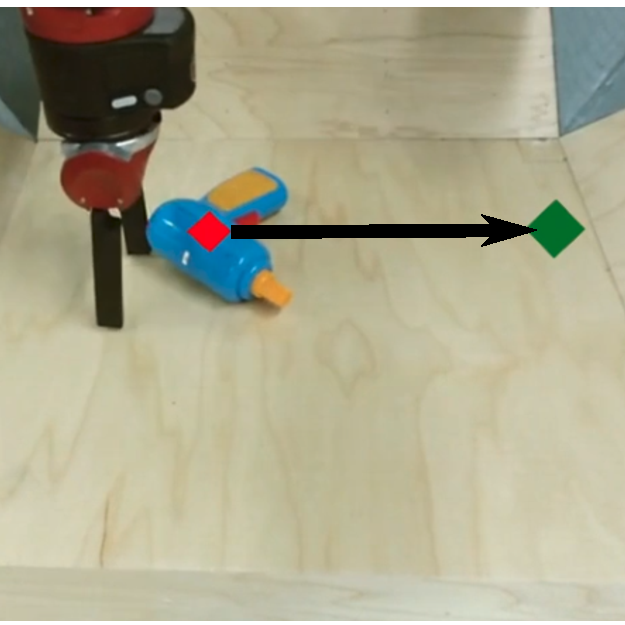
\includegraphics[width=0.30\columnwidth]{images_sna/longdistance_pushing/pushing.pdf}
	\caption{
		Pushing task. The designated pixel (red diamond) needs to be pushed to the green circle.
		\label{fig:long_distance_task}
	}
\end{wrapfigure}

We first perform a quantitative comparison of visual-MPC using the proposed occlusion-aware SNA video prediction model and the expected distance cost with visual-MPC using the dynamic neural advection model (DNA)\cite{foresight} with both the goal-point evaluation cost \ref{eq:goal_point_eval} and the expected distance cost \ref{eq:cost}.

We evaluate long pushes and multi-objective tasks where one object must be pushed without disturbing another. The supplementary video and links to the code and data are available at \url{https://sites.google.com/view/sna-visual-mpc}


\autoref{fig:long_distance_task} shows an example task for the pushing benchmark. We collected 20 trajectories with 3 novel objects and 1 training object. \autoref{table:res_dna_sna} shows the results for the pushing benchmark. The column \textit{distance} refers to the mean distance between the goal pixel and the designated pixel at the final time-step. The column \textit{improvement} indicates how much the designated pixel of the objects was moved closer to their goal (or further away for negative values) compared to the starting location. The true locations of the designated pixels after pushing were annotated by a human. 

The results in \autoref{table:res_dna_sna} show that our proposed planning cost in \autoref{eq:cost} substantially outperforms the planning cost used in prior work~\cite{foresight}. The performance of the SNA model in these experiments is comparable to the DNA model~\cite{foresight} when both use the expected-distance planning cost, since this task does not involve any occlusions. 
\begin{figure*}
\centering
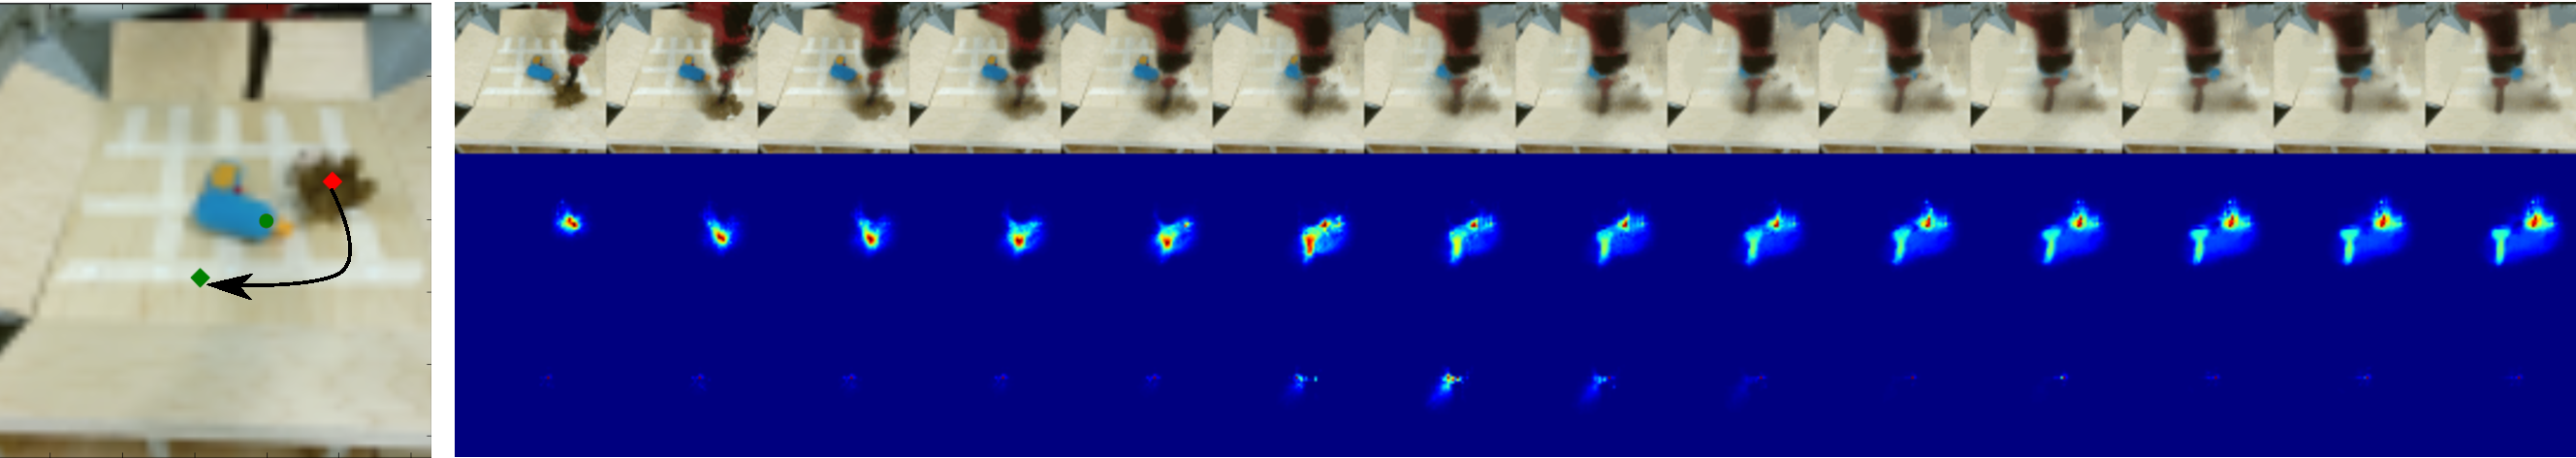
\includegraphics[width=1\linewidth]{images_sna/multiobject_qualitative/avoid_obstacle.pdf}
\caption{Left: Task setup with green dot marking the obstacle. Right, first row: the predicted frames generated by SNA. Second row: the probability distribution of the designated pixel on the \textit{moving} object (brown stuffed animal). Note that part of the distribution shifts down and left, which is the indicated goal. Third row: the probability distribution of the designated pixel on the obstacle-object (blue power drill). Although the distribution increases in entropy during the occlusion (in the middle), it then recovers and remains on its original position.
\label{fig:goingaroundocclusion}}
\end{figure*}

\begin{table}
{\footnotesize
    \begin{center}
    \begin{tabular}{lcc}
    	\toprule
           &  \thead{dist. \\ mean, std.} & \thead{improvement \\ mean, std.}  \\  
           \midrule
      DNA with cost eqn. \ref{eq:goal_point_eval}\cite{foresight}  & 24.6$\pm$10.6 & 2.1$\pm$12.4 \\
      DNA with cost eqn. \ref{eq:cost}  & \textbf{17.5 $\pm$ 10.2} &  \textbf{8.3 $\pm$ 11.8}\\ 
      SNA with cost eqn. \ref{eq:cost} (ours) & 18.18 $\pm$ 9.5 & 7.7 $\pm$ 10.5\\
      \bottomrule
    \end{tabular}
    \end{center}
    }
    \caption{Results of the pushing benchmark on 20 different object/goal configurations. Units are pixels in the 64x64 images.}
    \label{table:res_dna_sna}
\end{table}


\begin{table}
\centering
{\footnotesize
\begin{tabular}{lcc}
	\toprule
         &  \thead{moved imp. \\ mean, std.} &   \thead{stationary imp. \\ mean, std.}  \\
         \midrule
  DNA \cite{foresight} & 0.83 $\pm$1.13 &  -1.1 $\pm$ 0.9\\ 
  SNA & \textbf{10.6 $\pm$ 3.7} & \textbf{-1.5 $\pm$ 0.9} \\
  \bottomrule
\end{tabular}
}

\caption{Results for multi-objective pushing on 8 object/goal configurations with 2 seen and 2 novel objects. Values indicate improvement in distance from starting position, higher is better. Units are pixels in the 64x64 images.} 
\label{table:mult_obj}

\end{table}

%The pushing task evaluates the ability of each method to push an object across the table, but does not explicitly study the effect of occlusions. 
To examine how well each approach can handle occlusions, we devised a second task that requires the robot to push one object, while keeping another object stationary. When the stationary object is in the way, the robot must move the goal object around it, as shown in \autoref{fig:goingaroundocclusion} on the left. While doing this, the gripper may occlude the stationary object, and the task can only be performed successfully if the model can make accurate predictions through this occlusion. These tasks are specified by picking one pixel on the target object, and one on the obstacle. The obstacle is commanded to remain stationary, while the target object destination location is chosen on the other side of the obstacle.

We used four different object arrangements, with two training objects and two objects that were unseen during training. We found that, in most of the cases, the SNA model was able to find a valid trajectory, while the DNA model, that is not able to handle occlusion, was mostly unable to find a solution. \autoref{fig:goingaroundocclusion} shows an example of the SNA model successfully predicting the position of the obstacle through an occlusion and finding a trajectory that avoids the obstacle. These findings are reflected by our quantitative results shown in \autoref{table:mult_obj}, indicating the importance of temporal skip connections.

\subsection{Evaluating Closed loop Visual MPC}

\begin{table}
	{\footnotesize
		\begin{center}
			\begin{tabular}{lcc}
				\toprule
				%				 & \multicolumn{2}{c}{fraction of successful runs} \\
				& Short & Long \\
				\midrule
				Visual MPC $+$ predictor propagation  & 83\% & 20\% \\
				Visual MPC $+$ OpenCV tracking  & 83\%  & 45\% \\
				Visual MPC $+$ registration network & 83\% & \textbf{66\%}  \\
				\bottomrule
			\end{tabular}
		\end{center}
	}
	\caption{\small Success rate for long-distance pushing benchmark with 20 different object/goal configurations and short-distance benchmark with 15 object/goal configurations. Success is defined as bringing the object closer than 15 pixels to the goal, where the complete image has size 48x64.}
	\label{table:res_long_short}
\end{table}

Videos and visualizations for closed-loop visual MPC can be found on this webpage: \url{https://sites.google.com/view/robustness-via-retrying}. We compare visual-MPC that uses a pixel-distance based cost based on our proposed self-supervised registration with visual-MPC using an off-the-shelf tracker, the ``multiple instance learning tracker'' MIL \cite{babenko2009visual} from OpenCV. Note that all methods do not have any prior knowledge of objects -- it is only provided with the position of one designed pixel in the initial and goal images, and must use the learned model to infer that this pixel belongs to an object that can be moved by the robot. Finally we also compare to visual MPC without registration method proposed by \cite{sna}, which does not track the object explicitly, but relies on the flow-based video prediction model to keep track of the designated pixel, which we call ``predictor propagation.'' 

\subsubsection{Pushing with retrying}
\begin{figure*}
    \centering
    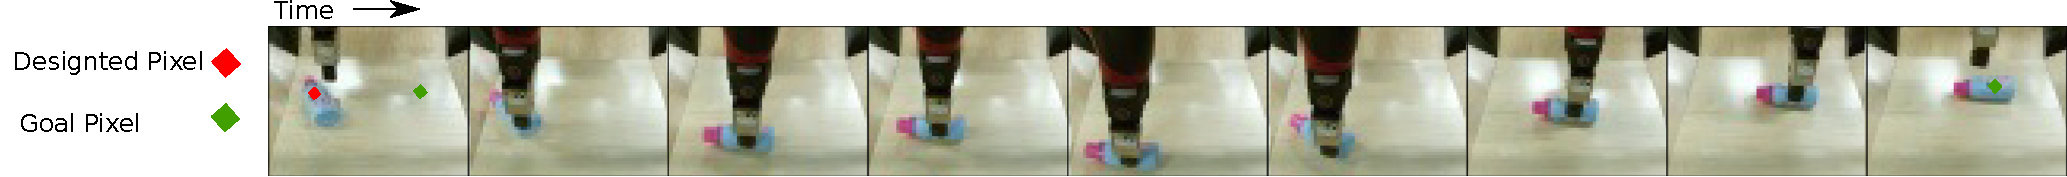
\includegraphics[width=1.0\textwidth]{images_rfr/push_correction.pdf}
    \caption{\small{Applying our method to a pushing task. In the first 3 time instants the object behaves unexpectedly, moving down. The tracking then allows the robot to retry, allowing it to eventually bring the object to the goal.}}
    \label{fig:push_retry}
\end{figure*}


%\begin{figure}
%	\centering
%	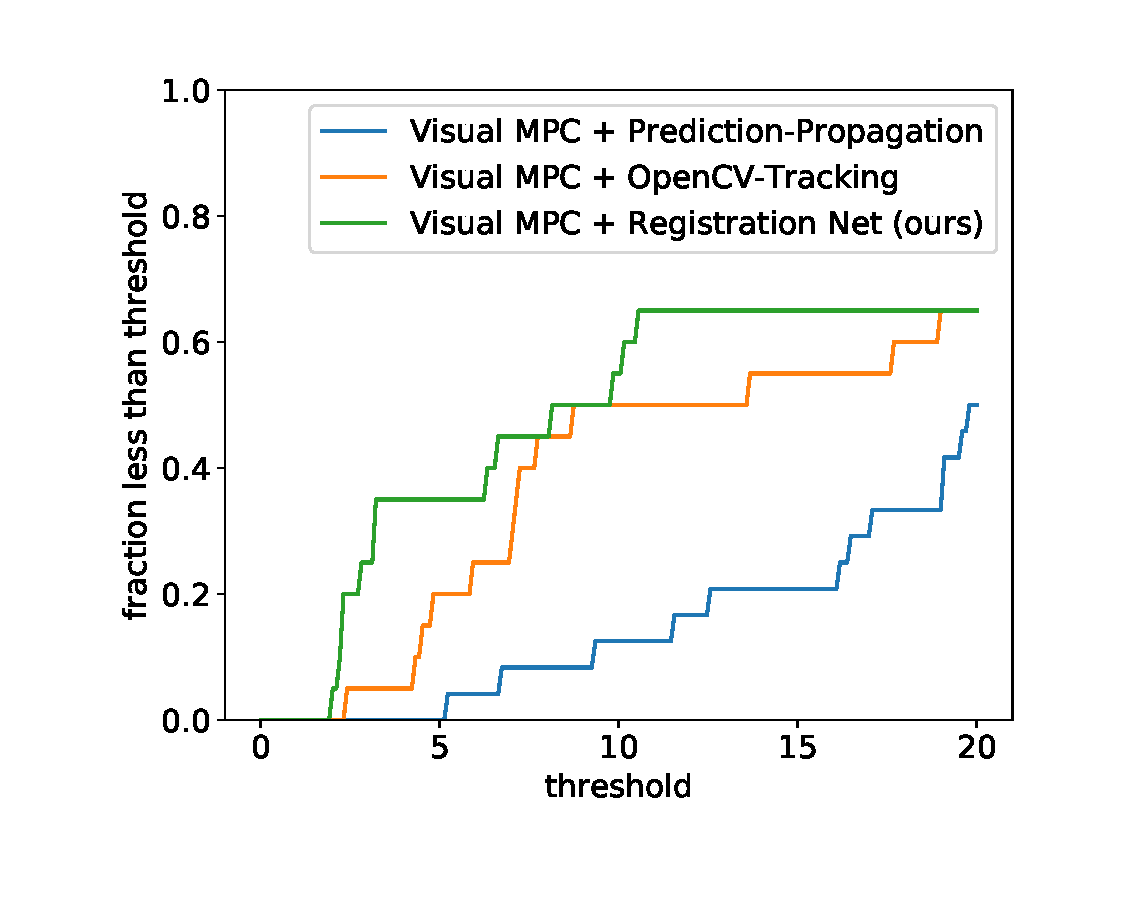
\includegraphics[width=0.8\columnwidth]{images_rfr/pushlong_bench_same_range.pdf}
%	\caption{\small{Results for long pushing tasks with 20 objects not seen during training, showing fraction of runs where final distance is lower than threshold. Our method shows a clear gains over OpenCV tracking and predictor propagation.}}
%	\label{fig:push_bench_long}
%\end{figure}

For the first experiment, we disable the gripper control, which requires the robot to push objects to the target. We evaluate our method on 20 long-distance and 15 short-distance pushing tasks. For long-distance tasks the distance between the object and its goal-position is $30cm$ while for short-distance tasks it is $15cm$. Table \ref{table:res_long_short} lists quantitative comparisons showing that on the long-distance benchmark visual-MPC using the proposed registrations approach not only outperforms prior work \cite{sna}, but also outperforms the hand-designed, supervised object tracker \cite{babenko2009visual}. By contrast for the short distance benchmark, all methods perform comparably. Thus theses results indicate the importance of closed loop control in long-horizon tasks. Using our learned registration, the robot is more frequently able to successfully recover after mispredictions or occlusions, an example is shown in \autoref{fig:push_retry}. 

%\begin{figure}
%	\centering
%	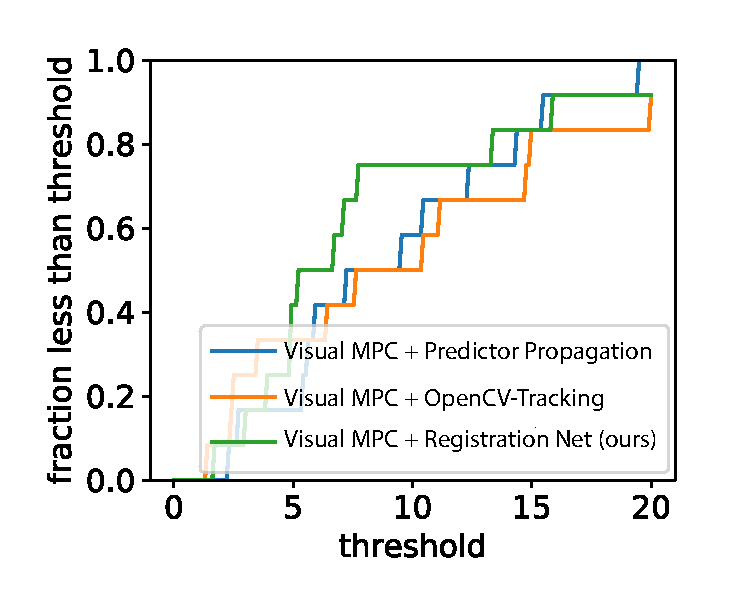
\includegraphics[width=0.8\columnwidth]{images_rfr/pushshort_bench_plots.pdf}
%	\caption{\small{Results for short pushing tasks.  Fraction of runs where final distance is lower than threshold.}}
%	\label{fig:push_bench_short}
%\end{figure}

\subsubsection{Combined prehensile and non-prehensile manipulation.}


In the setting where the gripper is enabled it is part of the task to decide whether to solve a task by grasping or pushing the object to the goal. Similarly to the pushing setting we perform a benchmark where we define a set of 20 object relocation tasks and measure the final distance between the object and the target at the end of the episode. Interestingly we observe that in the majority of the cases the agent decides to grasp the object, as can be seen in the supplementary video.

\subsection{Evaluating Classifier-based cost function}

For evaluating the performance of the proposed classifier-based cost function, we study a visual object arrangement task, where different goals correspond to different relative arrangements of a pair of objects. We evaluate our learned classifier on the predictions made by the video prediction model \todo{unclear, how exactly do you evaluate the classifier?} and derive the cost used for planning from the predicted probability of success.

\subsubsection{Real-World Experiments}

To collect data for meta-training the classifier, we randomly select a pair of objects from our set of training objects, and position them into many different relative positions, recording the image for each configuration. One task corresponds to a particular relative positioning of two objects, e.g. the first object to the left of the second, and we construct positive and negative examples for this task by labeling the aforementioned images. We randomly position the arm in each image, as it is not a determiner of task success. A good objective should ignore the position of the arm. We also include randomly-positioned distractor objects in about a third of the collected images.

We evaluate all approaches in three different experimental settings. In the first setting, the goal is to arrange two objects into a specified relative arrangement. The second setting is the same, but with distractor objects present. In the final, most challenging setting, the goal is to achieve two tasks in sequence. We provide positive examples for both tasks, infer the classifier for both task, perform MPC for the first task until completion, followed by MPC for the second task. To evaluate the ability to generalize to new goals and settings, we use novel, held-out objects for all of the task and distractor objects in our evaluation. 

We qualitatively visualize the evaluation in Figure~\ref{fig:qual_plan}.\todo{explain how exactly you measure success} On the left, we show a subset of the five images provided to illustrate the task(s), and on the left, we show the motions performed by the robot. We see that the robot is able to execute motions which lead to a correct relative positioning of the objects.
We quantitatively evaluate each method across 20 tasks, including $10$ unique object pairs. The results, shown in Figure~\ref{fig:planning_results}, indicate that prior methods for learning distance metrics struggle to infer the goal of the task, while our approach leads to substantially more successful behavior on average. 

% \begin{wraptable}{r}{0\columnwidth}
% \begin{tabular}{ll}
% \hline
% Method & Success Rate \\ \hline
% DSAE Distance & 10\% \\
% Pixel Distance & 20\% \\
% Classifier-based Cost & 75\% \\ \hline
% \end{tabular}
% \label{tbl:classifier}
% \end{wraptable}